%%%%
%       _  _____  ___  _____  _   _  ___ 
%      / \|_   _||_ _||_   _|| | | |/ __|
%     / △ \ | |   | |   | |  | |_| |\__ \
%    /_/¯\_\|_|  |___|  |_|   \___/ |___/
%                 EDUCAÇÃO
%    Modelo de TCC - Ciência da Computação
%%%%

\documentclass[12pt]{article}

\usepackage{sbc-template}
\usepackage{graphicx, url}
\usepackage[utf8x]{inputenc}
\usepackage[brazil]{babel}
\usepackage[T1]{fontenc}
\usepackage[english=american]{csquotes}
\usepackage{float}
\usepackage{comment}
\usepackage{amsmath}
\usepackage{amssymb}
\usepackage{enumerate}
\usepackage{subcaption}
\usepackage{setspace}
\usepackage{listings}
\usepackage{inconsolata}
\usepackage{tabularray}
%\usepackage[backref=page]{hyperref}
%\hypersetup{
%    colorlinks=true,
%    allcolors=blue,
%}

% %%%%%%%%%%%%%%%%%%%%%%%%%%%%%%%%%%%%%%%%%%%%%%%%%%%%%%%%%%%%%%
% define o modelo de referencias
\usepackage[style=abnt]{biblatex}

% indica o arquivo com as referencis bibliograficas
\addbibresource{sbc-template.bib}

% carrega o pacote com alterações para Computação Atitus
\usepackage{sty/cc_atitus}
% %%%%%%%%%%%%%%%%%%%%%%%%%%%%%%%%%%%%%%%%%%%%%%%%%%%%%%%%%%%%%%

% %%%%%%%%%%%%%%%%%%%%%%%%%%%%%%%%%%%%%%%%%%%%%%%%%%%%%%%%%%%%%%
% REFERENCIAS DEVERÃO SER INCLUÍDAS NO ARQUIVO: sbc-template.bib
%
% SOBRE CITAÇÕES:
% Para citar no padrão '(Autores, ano)' use: \cite{chave}
% Para citar no padrão 'Autores (ano)'  use: \textcite{chave} ou \citeonline{chave}
% Para citar no padrão 'Autores'        use: \citelastname{chave}
% Para citar no padrão '(Autor, 2009c; Outro Autor, 2009; Outro Autor, 2015)' use: \cites{chave1}{chave2}{chave3}
% Para citar no padrão 'Autor (ano), Autor (ano) e Autor (ano)' use: \textcites{chave1}{chave2}{chave3}

% Demais exemplos ver documento:
%  https://github.com/abntex/biblatex-abnt/raw/master/doc/biblatex-abnt.pdf
%
% Normas ABNT: https://usp.br/sddarquivos/arquivos/citacoes10520.pdf
%              https://usp.br/sddarquivos/arquivos/abnt6023.pdf
%
% %%%%%%%%%%%%%%%%%%%%%%%%%%%%%%%%%%%%%%%%%%%%%%%%%%%%%%%%%%%%%%
% Atualizações no modelo
% 2024-09-23: (fahadkalil) Ajuste para quebra automática de linhas nas células de uma tabela
% 2024-10-17: (fahadkalil) Inserção de comentários com outras citações e indicação de uso do comando "\enquote"
% %%%%%%%%%%%%%%%%%%%%%%%%%%%%%%%%%%%%%%%%%%%%%%%%%%%%%%%%%%%%%%
% CABEÇALHO
\title{Aplicação de Redes Neurais em Grafos para Aproximação da Métrica de Betweenness Centrality em Redes Sociais}

\author{Ana Luiza Almeida Soares\inst{1}, Rodrigo César Pedrosa Silva\inst{1}} % autor principal, orientador

\address{Programa de Pós-Graduação em Ciência da Computação \\ Departamento de Computação \\ Universidade Federal de Ouro Preto
\email{ana.almeida3@aluno.ufop.edu.br, rodrigo.silva@ufop.edu.br}
}
% %%%%%%%%%%%%%%%%%%%%%%%%%%%%%%%%%%%%%%%%%%%%%%%%%%%%%%%%%%%%%%

\begin{document}
\maketitle % Não remova essa linha!

% \begin{abstract} % resumo em inglês
%   Escreva seu resumo em língua estrangeira (inglês)...
% \end{abstract}
     
% \begin{resumo}
%   Resumo do trabalho (português)...  
% \end{resumo}

\section{Introdução}

As redes sociais têm se mostrado ferramentas poderosas para resolver uma ampla gama de problemas em diferentes áreas. Essas redes não se restringem apenas a plataformas digitais como Facebook, Twitter e Instagram, mas também são aplicáveis em contextos que envolvem interações entre elementos, como a disseminação de informações, a propagação de doenças, e a maximização de influência em campanhas de marketing. Sendo assim, em contextos como o espalhamento de notícias ou epidemias, a compreensão da estrutura da rede é crucial para prever e controlar o fluxo de informações ou patógenos.

Nessas aplicações, o peso das arestas desempenha um papel fundamental, uma vez que muitos algoritmos dependem dessa informação para operar de maneira eficiente. Por exemplo, o algoritmo de \textit{Linear Threshold} utiliza os pesos das arestas para determinar a probabilidade de um nó influenciar seus vizinhos, o que impacta diretamente o resultado do processo de propagação de influência. No entanto, obter essas informações de peso nem sempre é uma tarefa trivial, especialmente em redes grandes e complexas, onde esses valores podem não ser conhecidos ou fáceis de mensurar.

Uma abordagem comum para atribuir pesos às arestas em redes sociais é o uso da métrica de \textit{Betweenness Centrality}. Esta métrica mede a frequência com que uma aresta aparece nos caminhos mínimos entre todos os pares de nós na rede, sendo, portanto, um indicador de sua importância estrutural. No entanto, calcular a \textit{Betweenness Centrality} é um processo computacionalmente custoso, com complexidade \(O(n^2 m)\) em grafos não ponderados, onde \(n\) é o número de nós e \(m\) é o número de arestas. Isso torna o uso dessa métrica inviável para redes sociais de grande escala.

Diante desse desafio, o objetivo deste trabalho é utilizar uma \textit{Graph Neural Network} (GNN) para prever a \textit{Betweenness Centrality} das arestas em redes sociais, aproximando seu valor de forma mais eficiente. A proposta é explorar o potencial das GNNs para aprender padrões complexos de conectividade e fornecer estimativas precisas dessa métrica, reduzindo significativamente o tempo de processamento necessário em comparação aos métodos tradicionais.

% \section{Referencial Teórico}
% Voltado ao objetivo geral (teoria por trás do método), deve conter os assuntos bases da pesquisa, fazendo citações indiretas e diretas curtas.

% \begin{comment}
% testando comentario
% \end{comment}

% \begin{description}
%     \item[Exemplos de citação indireta]    
% \end{description}

% Segundo \textcite{spinello2024}, o trabalho de conclusão deve ter citações retiradas de artigos científicos encontrados nas bases de dados. 

% O trabalho de conclusão deve ter citações retiradas de artigos científicos encontrados nas bases de dados \cite{spinello2024}.

% \begin{description}
%     \item[Exemplos de citação direta curta]
% \end{description}

% Segundo \textcite{spinello2024} \enquote{o trabalho de conclusão deve ter citações retiradas de artigos científicos encontrados nas bases de dados}. Note que para colocar um texto entre aspas, usamos o comando \verb|\enquote{texto}|.

% Ressalta-se que o \enquote{trabalho de conclusão deve ter citações retiradas de artigos científicos encontrados nas bases de dados} \cite{spinello2024}.

% No estudo comparativo apresentado em \textcite[p. 107]{rabello2010} ...

% No trabalho de \textcite{pargaonkar2021} ...

% Nos trabalhos de \textcites{badgujar2024}{pargaonkar2021} são aplicadas técnicas de ...

% No artigo de \textcite{estevao2023} ...

% \textsc{Citação direta longa devem ser evitadas em artigos científicos!}

% \section{Trabalhos Relacionados}

% Trabalhos semelhantes aos objetivos específicos, sempre detalhando ao final da seção a
% diferença ao trabalho proposto (quantidade -- 5 trabalhos);

% Neste item serão apresentados os principais trabalhos que possuem uma relação com o assunto definido neste estudo....

% % Itens com marcadores
% \begin{itemize}
%      \item \textbf{Título do artigo 01 \cite{ogliari2019}}
     
%      Primeiro parágrafo indicar uma introdução do assunto... \\
%      No segundo: o que o estudo procurou analisar, qual o objetivo... \\
%      No terceiro: o que foi desenvolvido, qual aplicação/experimento foi realizado... \\
%      Último: em quais conclusões o trabalho chegou... \\
         
%     \item \textbf{Título do artigo 02 (Autor, ano)}
    
%      Primeiro parágrafo indicar uma introdução do assunto... \\
%      No segundo: o que o estudo procurou analisar, qual o objetivo... \\
%      No terceiro: o que foi desenvolvido, qual aplicação/experimento foi realizado... \\
%      Último: em quais conclusões o trabalho chegou... \\
    
%     \item \ldots
% \end{itemize}

\section{Materiais e Métodos}

A metodologia adotada para este trabalho envolve a escolha de três redes sociais, o cálculo da \textit{Betweenness Centrality} dessas redes, a seleção aleatória de algumas arestas com seus respectivos valores de \textit{Betweenness}, e a alimentação de uma \textit{Graph Neural Network} (GNN) com esses dados. Posteriormente, a previsão da GNN será comparada com os valores reais de \textit{Betweenness}, e o erro obtido será utilizado para avaliar a qualidade da previsão.

As redes sociais escolhidas para a experimentação foram obtidas a partir dos sites disponibilizados pelo Professor Dr. Vander Freitas na disciplina \textit{PCC 121 Redes Complexas}. Essas redes representam páginas do Facebook (verificadas, ou seja, páginas azuis) de diferentes categorias, e os nós representam as páginas enquanto as arestas representam as "curtidas mútuas" entre elas. Abaixo estão as redes selecionadas para o estudo:

\begin{enumerate}
    \item \textbf{Site:} \url{https://networkrepository.com/fb-pages-politician.php} \\
    \textbf{Nós:} 5.900 \\
    \textbf{Arestas:} 41.700
    
    \item \textbf{Site:} \url{https://networkrepository.com/fb-pages-food.php} \\
    \textbf{Nós:} 620 \\
    \textbf{Arestas:} 2.100
    
    \item \textbf{Site:} \url{https://networkrepository.com/fb-pages-artist.php} \\
    \textbf{Nós:} 50.500 \\
    \textbf{Arestas:} 819.100
\end{enumerate}

    % Tecnologias, instrumentos e procedimentos que serão usados no estudo. O Algoritmo \ref{alg:id_algo} se refere ao método de ordenação Bubblesort expresso em linguagem Python.

    % % Código-fonte formatado
    % % Ver: https://en.wikibooks.org/wiki/LaTeX/Source_Code_Listings
    % \begin{lstlisting}[  
    %     %float,
    %     language=Python, 
    %     frame=single, 
    %     numbers=left,
    %     caption={Método de ordenação Bubblesort},
    %     label={alg:id_algo} % id para referenciar
    %     ]        
    % def bubble_sort(alist):
    %     for i in range(len(alist)-1,0,-1):
    %         for j in range(i):
    %             if alist[i]>alist[i+1]:
    %                 temp = alist[i]
    %                 alist[i] = alist[i+1]
    %                 alist[i+1] = temp    
    % \end{lstlisting}

    % % Figura
    % % https://pt.overleaf.com/learn/latex/Inserting_Images
    % \begin{figure}[H]
    %     \centering
    %     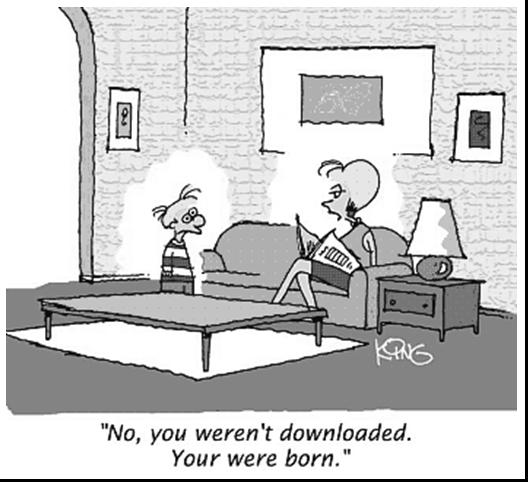
\includegraphics[width=0.5\textwidth]{fig1.jpg}
    %     \caption{Minha figura}
    %     \label{fig:id_figura}
    % \end{figure}
    
    % % Tabela
    % % Editor online: https://www.latex-tables.com
    %  \begin{table}[ht]
    %     \centering
    %     \caption{Minha tabela}
    %     \label{tab:id_tabela}
    %     \begin{tblr}{
    %       colspec = {X[l] X[l]}, % Tipo X define células com quebra automática de linha. Use: l=left, r=right, c=center ou j=justify para alinhamento dentro das células
    %       width = \linewidth,
    %       hlines, % inclui borda horizontal
    %       vlines, % inclui borda vertical        
    %     }
    %     \textbf{cabeçalho 1} & \textbf{cabeçalho 2} \\
    %     {texto à esquerda} & {Existem muitas variações das passagens do Lorem Ipsum disponíveis, mas a maior parte sofreu alterações de alguma forma, pela injecção de humor, ou de palavras aleatórias que nem sequer parecem suficientemente credíveis. Se vai usar uma passagem do Lorem Ipsum, deve ter a certeza que não contém nada de embaraçoso escondido no meio do texto.}
    %     \end{tblr}
    % \end{table}

\section{Resultados Esperados}

Espera-se que o erro entre a previsão da \textit{Graph Neural Network} (GNN) e os valores reais de \textit{Betweenness Centrality} não seja significativamente alto, indicando que a rede neural é capaz de aprender e generalizar bem as características da rede para estimar essa métrica de forma precisa. Além disso, espera-se que, ao utilizar a GNN para prever os valores de \textit{Betweenness}, haja uma melhoria considerável no tempo de processamento em comparação com o cálculo tradicional dessa métrica, que é computacionalmente custoso.


    

% \section{Considerações Finais}
% Essa seção deverá ser escrita na segunda parte do trabalho, conhecida como TCC2.

% %%%%%%%%%%%%%%%%%%%%%%%%%%%%%%%%%%%%%%%%%%%%%%%%%%%%%%%%%%%%%%
% Seção de Referências (gerada automaticamente)
\printbibliography  % Não remover esta linha
% %%%%%%%%%%%%%%%%%%%%%%%%%%%%%%%%%%%%%%%%%%%%%%%%%%%%%%%%%%%%%%

\end{document}